\Group{Tracking by Detection}

\begin{frame}
    \frametitle{How do we track an object from frame to frame?}
    \begin{columns}[T]
        \begin{column}{0.5\textwidth}
            \begin{figure}
                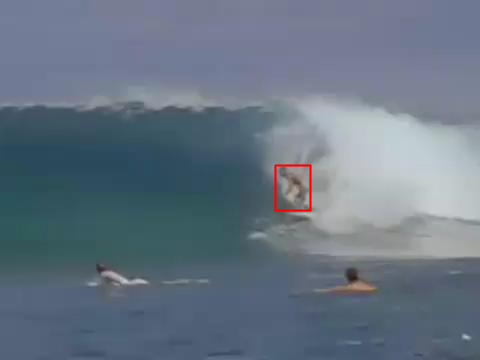
\includegraphics[width=0.9\textwidth]{surfer_marked}
                \caption{Initial frame: The surfer location is known.}
            \end{figure}
        \end{column}
        \begin{column}{0.5\textwidth}
            \begin{figure}
                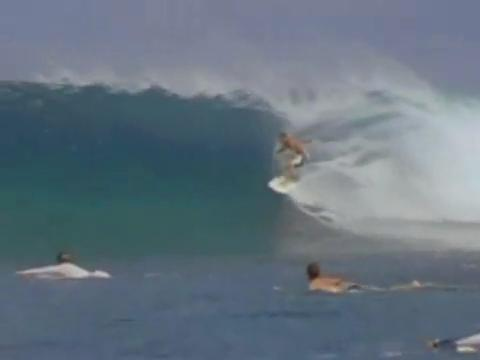
\includegraphics[width=0.9\textwidth]{surfer_unmarked}
                \caption{Subsequent frame: Where is the surfer?}
            \end{figure}
        \end{column}
    \end{columns}
\end{frame}

\begin{frame}
    \frametitle{What is tracking by detection?}
    \begin{description}
        \item [Tracking by detection] Attempt to detect the object in each frame.
    \end{description}
    \begin{itemize}
        \item Transform a tracking problem into an object detection problem.
        \item Can use prior knowledge to assist the detection.
            \begin{itemize}
                \item Previous position
                \item History of features
                \item For example, in the previous frame, the object was here. In this frame, it's
                    unlikely to be way over there.
            \end{itemize}
    \end{itemize}
\end{frame}

\begin{frame}
    \frametitle{General tracking by detection algorithm}
    \begin{itemize}
        \item The algorithm operates on frame \(f_t\), for \(t \in \{1, 2, ..., T\}\).
        \item Sample \(f_t\) around position \(\vec{p}_{t-1}\).
        \item Extract features \(\vec{x}_i\) for each sample.
        \item Input features to a classifier.
        \item Classifier determines which feature corresponds to the tracked object.
        \item Determine new position \(\vec{p}_t\).
        \item Retrain the classifier with new features. \alert{optional}
    \end{itemize}
\end{frame}

\begin{frame}
    \frametitle{Proposal: Fuzzy Struck}
    \begin{itemize}
        \item Fuzzy SVM incorporates fuzzy logic membership into an SVM. \cite{991432}
        \item Struck uses a structured output SVM. \cite{6126251} \cite{Schwenker2014}
        \item Overall, best performance in a recent survey. \cite{6671560}
        \item Two issues:
            \begin{itemize}
                \item Training samples often contain some object features and some background
                    features.
                \item Target object can change appearance over time, but this is not considered in
                    Struck.
                \item Tricky situation, though. What if the appearance changes, then reverts back to
                    the original?
            \end{itemize}
        \item Combine fuzzy SVM with Struck's SVM.
    \end{itemize}
\end{frame}
